% ---------------------------------------------------------------------------
% August 6 session: regime transfer, the simulation program, anatomy of a
% false certification, and the release rule.  Inserted 2026-08-06.
% ---------------------------------------------------------------------------
\section{August 6 session: regime transfer, known-truth simulation, anatomy of a false certification, and the release rule}\label{sec:aug6}

This section records a single extended session (August 5--6, 2026) on the 2020
COVID refi-wave regime and on the certification machinery itself. Its
deliverables: (i) a two-regime panel with a standing \emph{law fixed-point per
regime} rule and one retraction; (ii) a known-truth simulation program that
calibrates the solver's reported uncertainty and adjudicates the shrinkage
design; (iii) a complete causal account of one false certification, from
admission through redistricting to repair, with the constrained-closure
mechanism and its local-release cure demonstrated on real data; (iv) a
release-rule design with full-mesh censuses, a two-currency principle with
measured teeth, and a first working hierarchical (two-groups) trust layer that
produces the best held-out surface of the session. Status labels throughout:
\textsc{measured} (numbers from data or simulation), \textsc{design} (agreed
specification, not implemented), \textsc{retracted}.

\subsection{The 2020 regime: transfer, the law fixed point, and a retraction}
\label{sec:aug6-regime}

\textsc{Measured.} All twelve 2020 monthly SFPS files parse and transport
cleanly (225--238k pools/month, 11 transitions, zero negative loan-count
drops). Wave-regime persistence is structurally different from 2026:
attenuation-corrected signal correlations $0.795/0.651/0.570/0.487$ at lags
$1/2/3/6$ imply a near-fixed frailty component ($\approx$45--50\% of signal)
against 2026's AR$(1)$-like $\rho\approx0.65$; signal is 75\% of pool residual
variance in both regimes. The stage-boosting chain transfers with a frozen
tournament ordering and per-month stage gates, with gains 2--3$\times$ the
2026 scale.

\textsc{Retracted.} The initial finding that the chain \emph{loses} the
June$\to$July and July$\to$August 2020 transitions (the delinquency-buyout
months) was a law artifact. Refitting the SMM pool-law fixed point on the 2020
regime (per-stratum totals $0.151/0.254/0.126/0.049$ against 2026's
$0.143/0.242/0.029/0.004$; the mega-pool strata carry $4$--$13\times$ the 2026
variance) and re-running gates and scoring under the 2020 law flips
June$\to$July to a $+0.093$ NLL win. The buyout-months story is downgraded to
at-most-deviance-neutral. Standing rule: \emph{the law fixed point is
per-regime and per-model} (including post-boosting refits; the boosted chain
absorbs $\approx$77\% of pool-effect variance, leaving the 2026-calibrated law
$\approx4\times$ too large); pinning a law across regimes converts law
misspecification into fake structural conclusions.

\subsection{Known-truth simulation and the honest-uncertainty stack}
\label{sec:aug6-sims}

Two worlds built on the real January-2026 design geometry (real coupon
lattice, sizes, issuer labels; truth surface from a fitted field): world A
with the exchangeable converged law; world B with issuer-block effects (sd
0.30) plus a reduced individual law. \textsc{Measured} verdicts:

\begin{itemize}[leftmargin=2em,itemsep=2pt]
\item \textbf{The reported $\sigma^2$ is optimistic everywhere.} Claimed
coefficient standard errors understate realized error $2.21\times$ in the
\emph{perfectly specified} world A (joint-fit correlation plus selection) and
$3.18\times$ under blocks. The dominant term is joint-fit correlation, not
winner's curse: reading contrast variances off the full penalized-information
inverse restores $\mathrm{sd}(z_{\mathrm{err}})=1.13$ in world A; adding a
law-plus-block sandwich $\Omega$ restores $1.12$--$1.35$ in world B.
\item \textbf{Gate error rates.} False admissions 27\% in world A (an upper
bound under the approximate null definition), 36\% under blocks. A two-groups
audit on sandwich-honest $z$'s removes 42--45\% of false admissions at
85--87\% retention; the same audit on claimed $\sigma^2$ removes 6\%.
\item \textbf{Coarseness is the identifiability defense.} Only 5\% of the
injected block effect leaks into the fitted surface (13\% for spatially
concentrated blocks, 3\% diffuse); the mesh refuses blocks to the pool layer
and the law prices what is refused. Block-aware nulls are targeted cleanup,
not global repair; the pool-layer/panel treatment is where refused variance
becomes forecastable signal.
\item \textbf{The fair fight.} Frozen-topology joint re-solves differing only
in $\Lambda$: depth-based shrinkage ties the honest two-groups prior for point
estimation in both worlds (oracle wMSE $0.0156$ vs $0.0154$;
$0.0455$ vs $0.0448$). Sophistication's proven value is calibrated
uncertainty and audit power, not primary-plane point estimates.
\item \textbf{Post-hoc coordinatewise re-shrinkage is refuted.} Applying
audit-derived shrinkage marginally degrades the surface catastrophically
(world A oracle wMSE $0.033\to0.159$): coefficients are fitted jointly and
their errors cancel; marginal edits break the cancellation. Shrinkage may
enter only through $\Lambda$ inside the joint solve.
\end{itemize}

Separated deliverables: (a) in-loop se fix (contrast variances off the
existing factorization, sandwich $\Omega$) --- ship; (b) two-groups $q$'s as a
post-hoc \emph{audit} overlay --- usable now; (c) prior upgrades in-loop only;
(d) post-hoc surface editing --- never.

\subsection{Anatomy of a false certification}\label{sec:aug6-anatomy}

The June$\to$July 2020 fit certifies a $+4.43$-logit surplus ($9\sigma$
against reported se, trust $T=0.95$) at a coupon-lattice corridor vertex,
rendering 25.2\%/month over pools whose hat-weighted evidence is
1.09\%/month. The session traced this object end to end; every intermediate
hypothesis was tested and most died.

\paragraph{Static forensics (\textsc{measured}).} The vertex's heavy voters
are zero-event pools ($k=0/43,0/84,0/63,\ldots$); the fast pools in its ring
are low-hat fringe members of neighboring coupon columns. The lineage
sawtooths ($-2.20$, $-2.01$, $+4.43$, each ``significant'' marginally,
jointly a modest field): coordinatewise audits certify teeth, not the bite.
A one-coordinate height sweep under the tail law leaves 23.8 nats on the
table (31.5 binomial) against the parent level. Eliminated: robustness
plateau, prior anchoring (prior means are zero for all 118 admissions),
dump-column confusion (the \texttt{height} column reproduces shipped
$\hat p$ to $R^2=1.000000$), staleness (a final exact frozen-topology refit,
\texttt{DMESH\_HIER\_FIT=2}, moves nothing), and temper distortion (a
law-GLS re-tempered final solve, \texttt{DMESH\_LAW\_WEIGHTS\_FINAL=1},
moves \emph{other} vertices but not this one).

\paragraph{Mechanism: the constrained-closure compromise (\textsc{measured}).}
The vertex carries four conformity-welded midpoint descendants (no
coefficients), so its exact design column spans a footprint of 36 extra train
pools (1{,}872 loans at 5.50\%/month) beyond its one-ring (18 pools, 749
loans, 2.67\%/month). The hot constrained footprint outvotes the corridor;
the compromise is rendered where the losing population lives; the solver is
converged. One knob, two rooms (Figure~\ref{fig:aug6-tworooms}). This is the
third basis-level disease after boundary anisotropy and lattice voids, and it
has a certification corollary: \emph{a certificate must quote a coefficient's
footprint through its constrained children, not its one-ring}.

\begin{figure}[t]
\centering
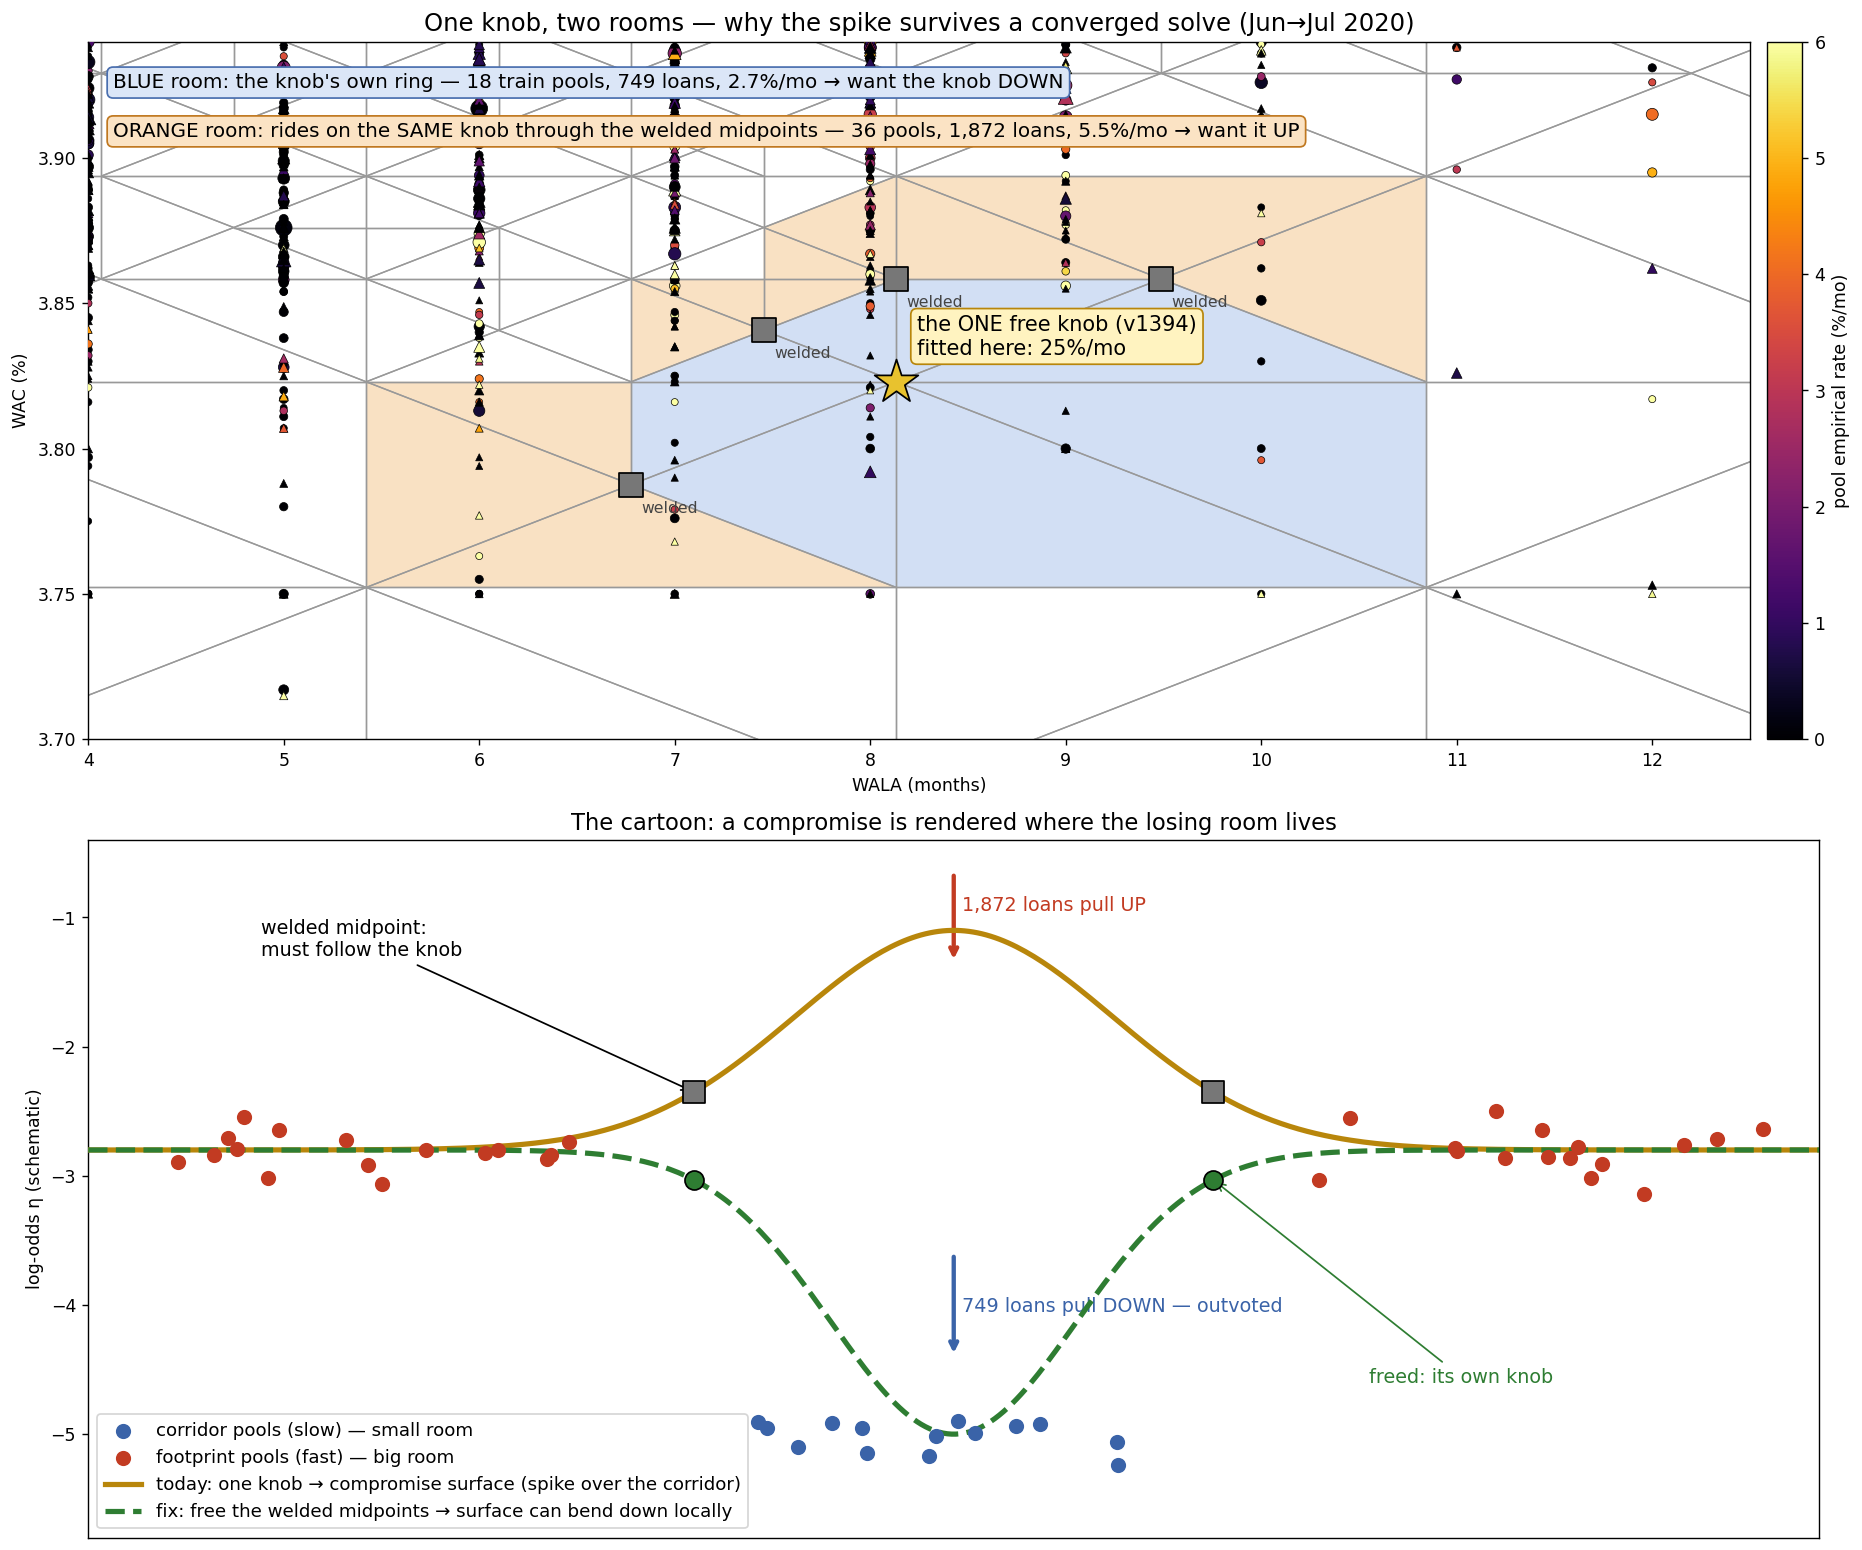
\includegraphics[width=0.92\textwidth]{one_knob_two_rooms.png}
\caption{The constrained-closure compromise. Top: the real region; marker
area is vote share at the certified vertex, color is empirical rate; the
one-ring (blue room) wants the coefficient down, the constrained footprint
(orange room) rides the same coefficient through welded midpoints and wants
it up. Bottom: schematic; the compromise surface is rendered over the losing
room, and freeing the welded midpoints lets the surface bend.}
\label{fig:aug6-tworooms}
\end{figure}

\paragraph{History: the gerrymander (\textsc{measured}).} Round-capped
snapshot refits (\texttt{DMESH\_MAX\_GATE\_ROUNDS} +
\texttt{DMESH\_STOP\_AFTER\_ADAPTATION}, vertex tracked by coordinates)
recover the biography (Figure~\ref{fig:aug6-filmstrip}): promoted at round 5
at $\eta=-1.82$ serving 97 pools/5{,}934 loans at 3.6\%/month (raw data pull
$+0.82$ logits; defensible); successive refinements carve the ring
$97\to48\to26\to18$ pools with pooled rate swinging
$3.6\to5.2\to8.2\to2.7$\%/month; the height never re-adjusts while welds
accumulate one to five. Elected by one constituency, redistricted into its
opposite, prevented from resigning. The one-coordinate relax dual (below)
already reads $+14.6$ train / $+35.4$ held nats at round 5: the compromise
predates the carving, and a per-carve ``redistricting review'' would have
flagged it five rounds early.

\begin{figure}[t]
\centering
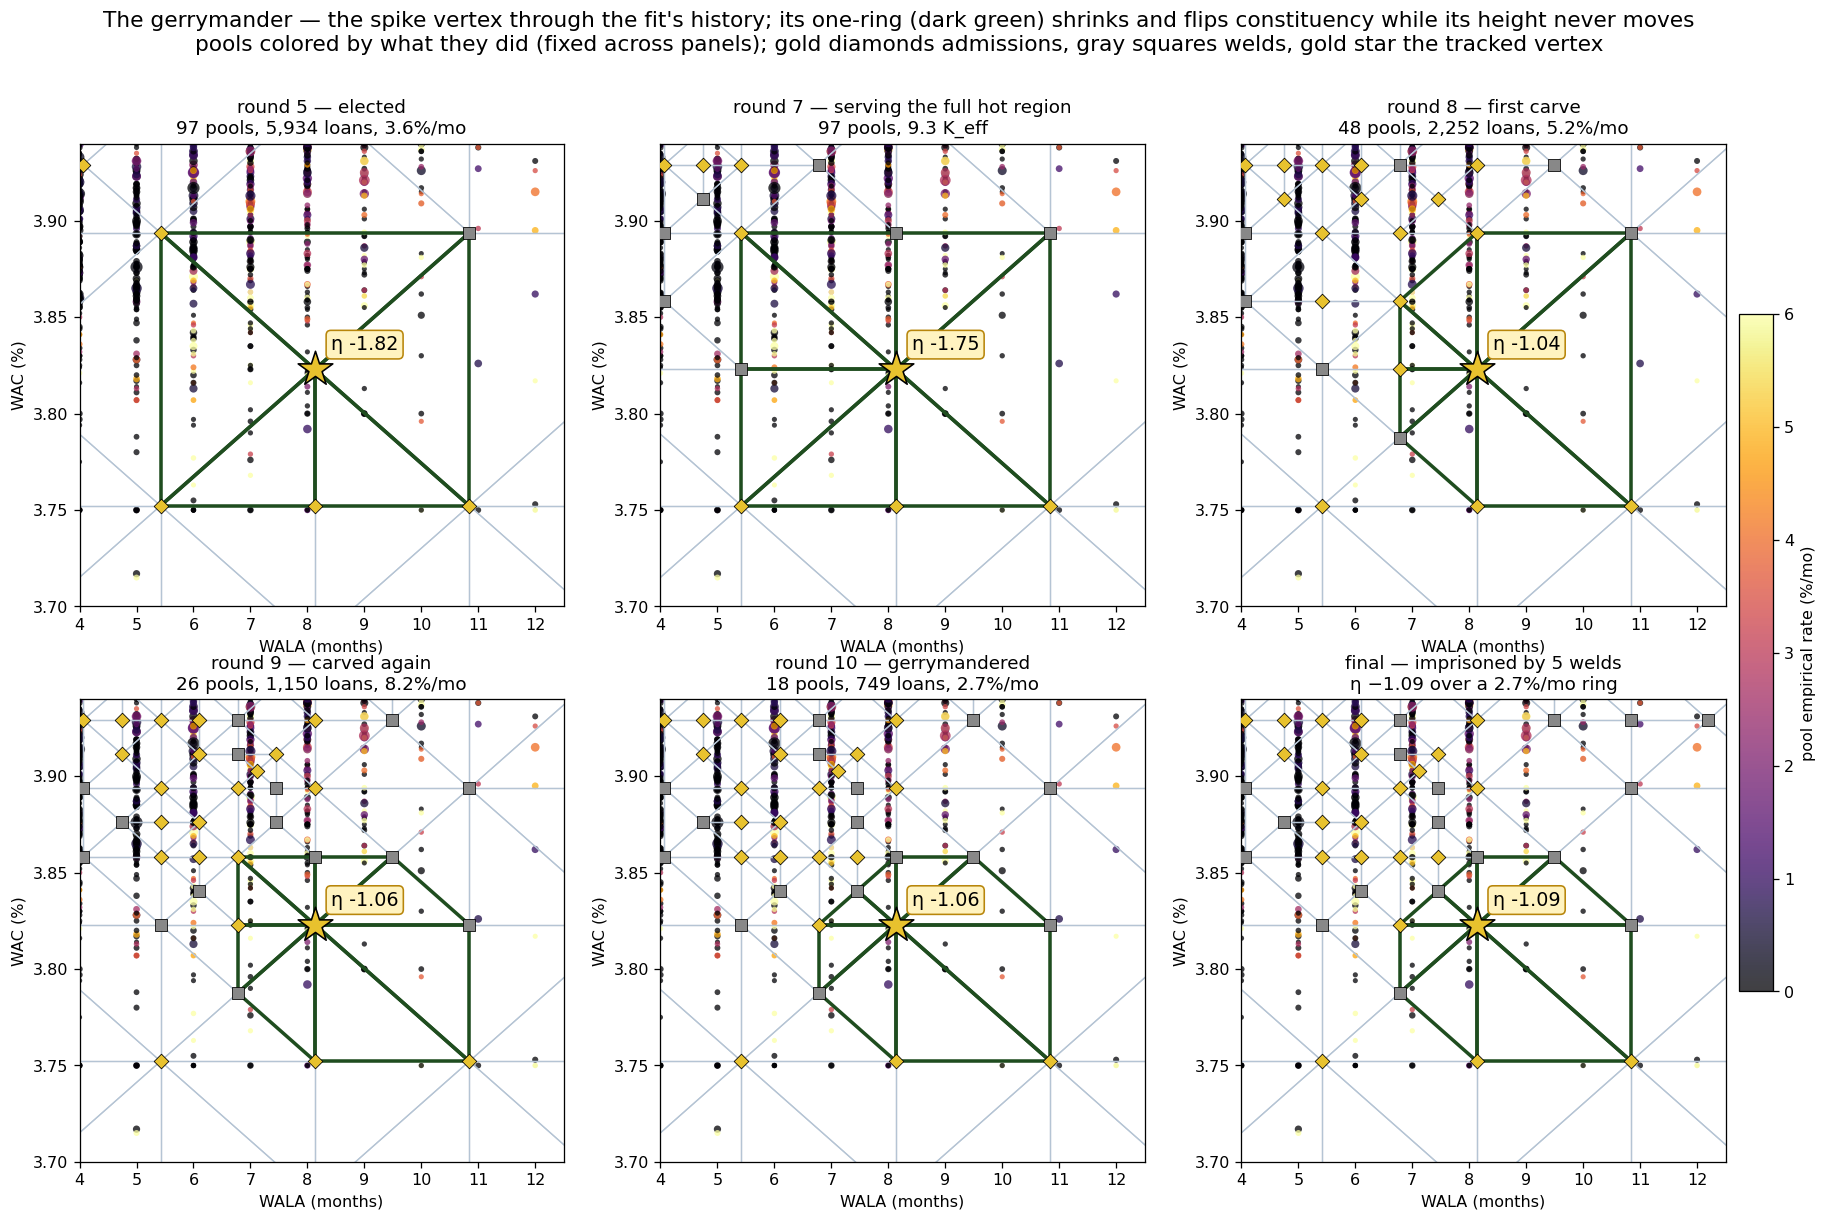
\includegraphics[width=\textwidth]{spike_history_filmstrip.png}
\caption{The gerrymander. Six exact snapshots of the region; the tracked
vertex's one-ring (dark green) shrinks and flips constituency
(3.6$\to$5.2$\to$8.2$\to$2.7\%/month) while its height stays fixed and welds
(gray) accumulate.}
\label{fig:aug6-filmstrip}
\end{figure}

\paragraph{Repair: local release (\textsc{measured}).} Freeing the four welds
and re-solving only those five heights (coordinate ascent on the law-marginal
train likelihood, $\tau=1$-logit prior toward parent interpolation,
everything else frozen): the knob moves $-1.09\to-4.42$, landing at the
ring's hat-weighted evidence ($-4.50$; the pre-registered bar was ``$-4.5$
or below,'' missed by 0.08 and flagged); region train likelihood $+31.5$
nats, \emph{held-out} $+37.9$ nats. The blue room's 16 held-out pools go
from deviance 6.27 (2.2$\times$ the month average) to 1.37 (better than
average); the orange room's held-out $z$ improves $-1.87\to-0.57$; full-month
held-out deviance improves $+0.0049$ from five numbers
(Figure~\ref{fig:aug6-after}).

\begin{figure}[t]
\centering
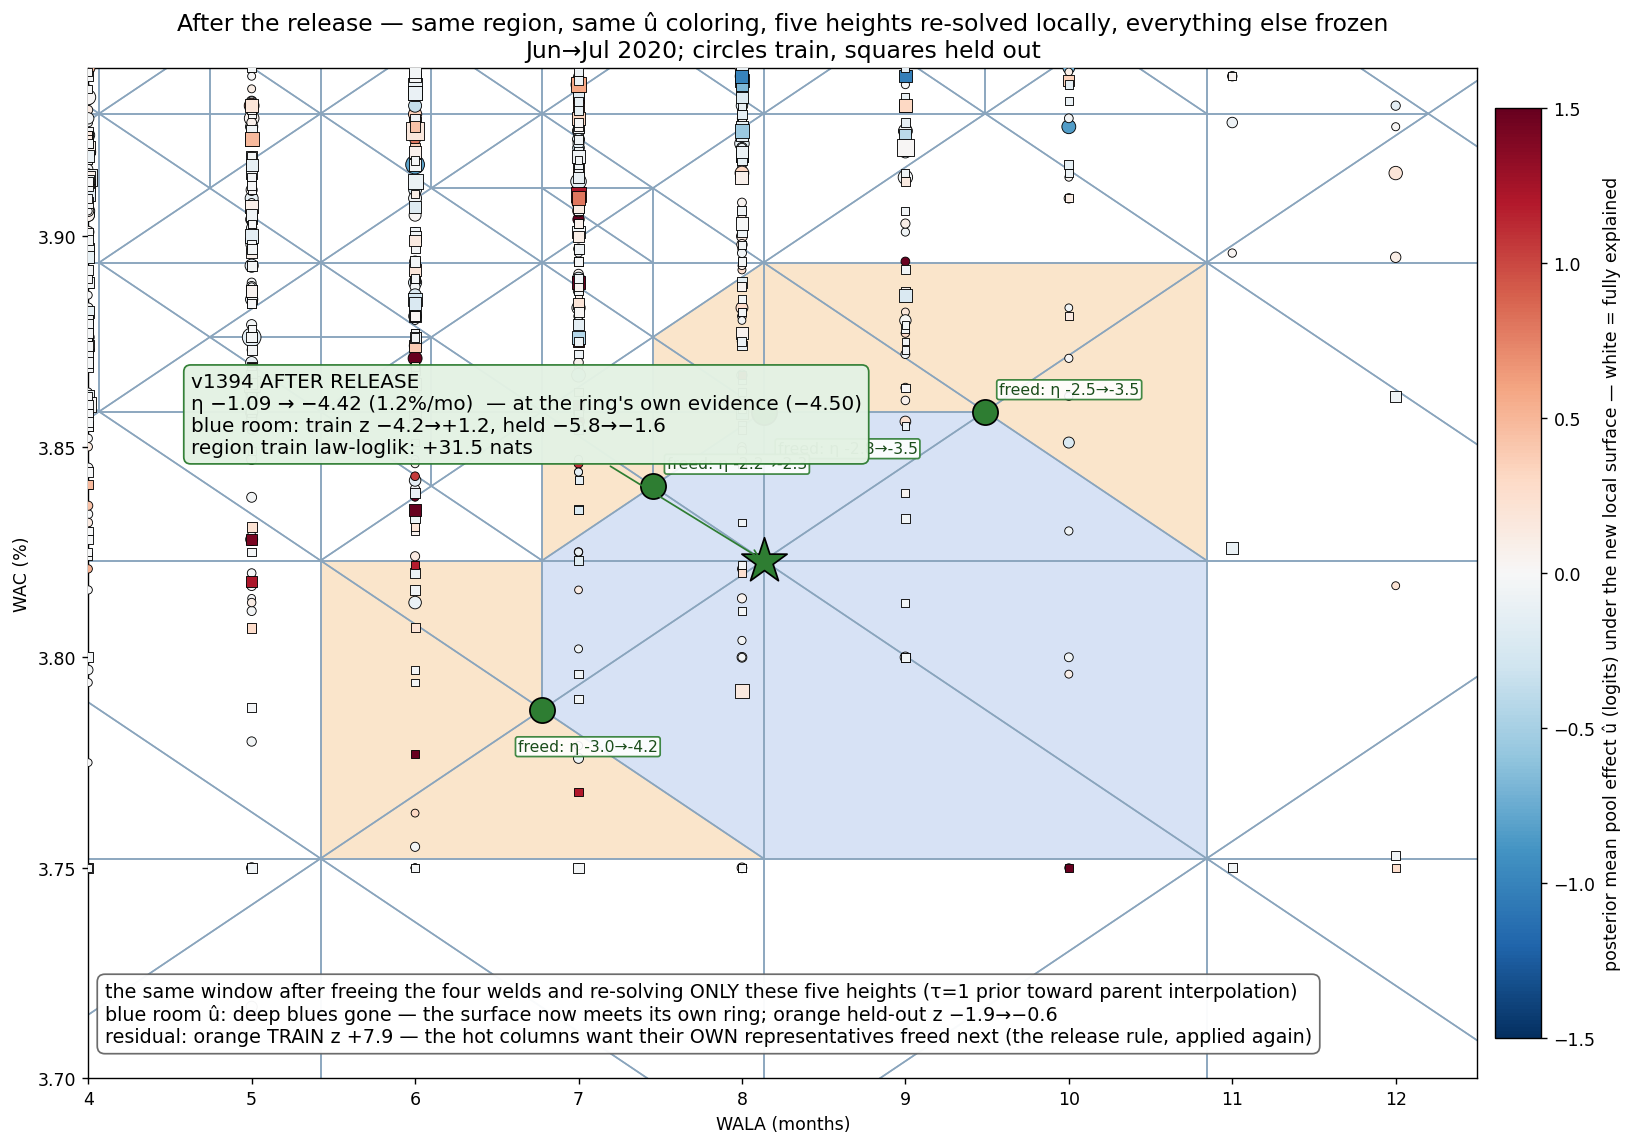
\includegraphics[width=0.94\textwidth]{void_spike_after_release.png}
\caption{After the five-height local release: credibility posteriors
$\hat u$ under the new local surface. The coherent blues under the certified
vertex are gone; the freed midpoints (green) settle at their own rooms'
levels.}
\label{fig:aug6-after}
\end{figure}

\subsection{The release rule, the censuses, and the two-currency principle}
\label{sec:aug6-release}

\paragraph{Design (\textsc{design}, agreed).} Welded midpoints and unproposed
candidates are the same object: linearity constraints. Decouple geometric
status \{absent, present-conforming\} from statistical status \{constrained,
free\}, price every constraint by its one-ring score multiplier through the
same gate (releases enter the e-BH budget; winner's curse applies), allow
release and re-weld transitions, re-audit footprints and re-score greedily
between releases, and trigger re-pricing on every ring-changing refinement.

\paragraph{Censuses (\textsc{measured}).} Weld census, June$\to$July: 119
welds, 99 scoreable; 16 fire at $|z_{\mathrm{ring}}|>3$; 11 replicate
held-out (the honest docket), 3 are train-only flip/flicker suspects (a
labeled test set for the block-aware null), 83 quiet. Firing welds have
median rings of 41 pools/3{,}045 loans: the multiplier self-protects against
voids. Full relax census (one-coordinate relaxed fit and nat gain, fitted on
train and scored on both halves, all 270 scoreable vertices,
Figure~\ref{fig:aug6-census}): the naive ``both halves $>5$ nats'' docket is
55 vertices (20\%) but is \emph{confounded}; decomposing by intensity
(held nats per ring pool) splits it into a \textsc{diffuse} class (36
vertices, median shift $-0.86$ logits, median ring 1{,}071 pools, 0.036
nats/pool) and a \textsc{sharp} class (19 vertices, 7\%, median shift
$-2.21$, median ring 61 pools, 0.25 nats/pool) clustered exactly at the two
known disease loci: 13 of 19 in the corridor complex, plus the issuance
boundary.

\begin{figure}[t]
\centering
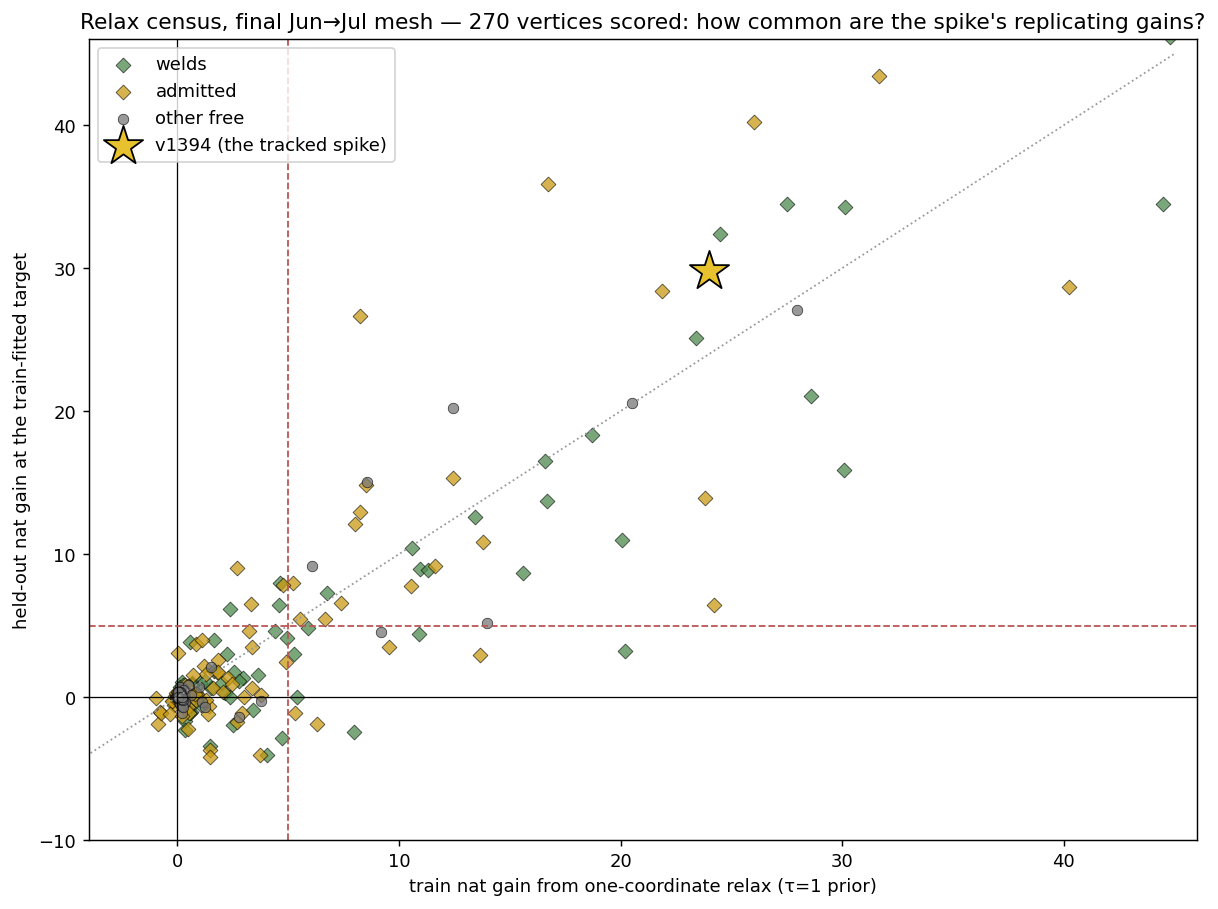
\includegraphics[width=0.8\textwidth]{relax_census_final.png}
\caption{Relax census on the final mesh: train versus held-out nat gain of
each vertex's one-coordinate relaxed fit. The replicating extreme class is
rare and clustered; the tracked vertex is the star.}
\label{fig:aug6-census}
\end{figure}

\paragraph{The two-currency principle (\textsc{measured}).} The diffuse class
is an artifact of scoring in the wrong currency. The relax criterion used the
law-\emph{marginal} likelihood; the solver ships the \emph{conditional}
surface; logit-normal attenuation puts the marginal-ML location
$\approx\frac12\sigma^2$ lower everywhere. Jointly refitting all 30 vertices
with $>20$ train nats (15 of them welds) executes this recalibration on 71\%
of the book and grades oppositely under the two currencies: held-out
deviance $2.794\to3.516$ (disaster) while held-out mixture NLL
$1.697\to1.644$ (the largest single improvement of the session). Pricing the
convexity into the prediction ($\bar p=\mathbb E[\mathrm{expit}(\eta+u)]$)
recovers only 0.11 of the 0.72 deviance gap: convexity is $\approx$15\% of
the wedge; the residual is the heavy-tail marginal acting as a \emph{robust
location estimator} (pulled toward the median pool) while mean prediction
needs the exposure-weighted mean --- i.e., the law books persistent fast
subpopulations as exchangeable tail noise, and the residual is the measured
prediction-space price of that misspecification. Consequences: the release
objective must be stated in the conditional/working currency for the
deployment target; the marginal surface-law fixed point is a research object
for distributional consumers; and $\mathrm{dev}(\bar p)$ joins the toolkit as
a \emph{currency detector} (the sign of $\mathrm{dev}-\mathrm{dev}(\bar p)$
identifies which optimum a surface occupies).

\paragraph{Three-currency scoreboard (\textsc{measured}, held-out,
June$\to$July).}

\begin{center}
\begin{tabular}{lccc}
\hline
surface & dev & dev$(\bar p)$ & mixture NLL\\
\hline
shipped & 2.7936 & 2.8347 & 1.69734\\
5-vertex local release & 2.7890 & 2.8297 & 1.69544\\
sharp-class release (19v, ad-hoc cut) & 2.7748 & 2.8013 & 1.67916\\
bulk $>$20-nat refit (30v) & 3.5155 & 3.4024 & 1.64405\\
hierarchical-$\tau$, marginal duals (128v) & 4.1713 & 4.0371 & 1.63238\\
hierarchical-$\tau$, conditional duals (66v) & \textbf{2.7355} & \textbf{2.7694} & 1.68570\\
\hline
\end{tabular}
\end{center}

The sharp-class release is the first intervention of the session to improve
all three currencies simultaneously; the conditional-dual hierarchical-$\tau$
release (below) then triples its deviance gain. Both carry mild selection
tint (held-out-informed cuts) and await fresh-seed confirmation.

\subsection{Stuckness, the ladder, and the hierarchical trust layer}
\label{sec:aug6-ladder}

\paragraph{Why geometry sticks (\textsc{measured} taxonomy).} Classifying the
19 sharp sites by mechanism (constrained descendants; trust and stiffness;
whether the law-GLS exact refit moves them): 5 are welds themselves; 6 are
closure-coupled free vertices (two rooms); 6 are \emph{soft-welded} free
vertices; 1--2 are temper-priced or joint-direction (valley) cases. The soft
welds are the discovery: $\lambda_v=10^8$ \emph{uniformly} across all 49
depth-8/9 admissions ($\lambda\sigma^2\sim10^{10\text{--}11}$, $T=0$,
rendered surpluses $\approx0$), against $\lambda\sim10^{-4}$ at depths
$\le7$: the fitted ladder is binary, free through depth 7 and welded from
depth 8. The clearest victim (v1599, depth 8) has $\sigma^2=7.3$
centilogit$^2$ --- excellent information --- and is pinned anyway. Bug lead:
with \texttt{DMESH\_TAU\_FLOOR\_LOGIT\_SD=0.005} the floor implies
$\lambda\le4$; depth 10 shows exactly $\lambda=4$ (floor working) while
depths 8--9 show $10^8$ (floor bypassed; sentinel or defect --- source read
queued). Unifying statement: evidence accumulates in nodal directions,
stiffness is levied in hierarchical ones; hard welds ($\lambda=\infty$), the
ladder's wholesale welds ($\lambda\to10^8$), and closure-coupled parents are
one Lagrangian phenomenon, and the principled repair is to make every
stiffness priceable by a dual (the whitened, conditional-currency,
footprint-aggregated score) with release and re-weld transitions under the
certification budget.

\paragraph{Hierarchical $\tau$, first working version (\textsc{measured}).}
A per-tier two-groups EM on the relax duals (tiers: free $\le d7$, free
$d8{+}$, welds; statistic: log train nats per ring pool; slab requires
posterior $>0.5$ and positive held-out gain), followed by a joint local
release of the slab. Fed \emph{marginal}-currency duals the EM selects 128
vertices (the attenuation field is a real nonzero signal in that currency)
and produces the worst deviance of the session (4.1713). Fed
\emph{conditional}-currency duals (plain binomial ring likelihood) it selects
66 vertices --- the corridor knob in, the diffuse giants out, 57 sites beyond
the ad-hoc sharp cut --- and produces the session's best surface on both
deviance currencies (table above). Same prior, same release machinery; only
the dual's currency changed. Caveats: the shallow-tier mixture separation is
weak (slab mean 0.006 nats/pool; near the two-cluster degeneracy),
posterior-threshold sensitivity and fresh-seed confirmation are required.

\paragraph{EB shrinkage, conceptual audit (\textsc{design}).} What is right:
the parent-interpolation null and per-scale variance decay. Four structural
defects, each with a session exhibit: (1) depth is the wrong exchangeability
unit (one $\tau$ spans K$_{\mathrm{eff}}$ 0.01 corridors and K$_{\mathrm{eff}}$
100 workhorses: the wholesale weld and the weak-plane self-licensing are the
two failure directions of the same choice); (2) the learning signal is
corrupted (fitted, entangled coefficients teach the ladder the solver's
ringing; gate truncation; working-binomial noise denominators understate by
2--3$\times$, and understated noise means overstated signal variance exactly
where noise is worst); (3) the gate and the ladder are two disconnected
inferences on the same hypothesis --- 49 of 118 gate-admitted coefficients
carry $\lambda=10^8$, admitted by one organ and welded by the other; the
correct object is a single spike-and-slab posterior per cell whose slab
probability \emph{is} the admission quantity and whose slab variance
\emph{is} the shrinkage; (4) the application point: compound-loss optimality
for coefficients is not optimality for the field; shrinkage enters only
through $\Lambda$ in the joint conditional-currency solve. Target design, all
components individually validated this session: spike-and-slab per
(depth $\times$ evidence-geometry) cell, fitted by g-modeling on whitened
coefficients or data-side duals over the full candidate ensemble including
refusals, sandwich-honest denominators, unified with the gate, applied
in-loop, re-priced on design-changing events. The measured bar for the
in-loop implementation is the conditional-dual release's 2.7355.

\subsection{Session open-item delta}\label{sec:aug6-open}

New or re-ranked relative to Section~\ref{sec:discussion}: (1) the release
rule and redistricting review (in-loop; conditional currency; e-BH budget);
(2) the \texttt{TAU\_FLOOR} bypass at depths 8--9 (bug read); (3) in-loop
two-groups $\Lambda$ with the marginal Newton, bar 2.7355; (4) sandwich se
inside the exact scorer (unchanged, still first); (5) fresh-seed confirmation
of the sharp-class and conditional-slab releases; (6) the 11-site weld docket
with pre-registered targets, and the 3 train-only firings as the block-null
test set; (7) exact-age dummies or anisotropic refinement at the issuance
boundary (unchanged); (8) the marginal surface-law fixed point as a
research note for distributional consumers.
